\documentclass[british,titlepagevegard,oneside]{ntnuthesis}

\newcommand{\todo}[1]{\textcolor{red}{TODO: {#1}}}

\title{Comparison of two classical landmark detectors for side scan sonars}
\shorttitle{Comparison of landmark detectors}
\author{Vegard Haraldstad}
\shortauthor{Haraldstad}
\date{\today}

\addtolength{\oddsidemargin}{-.875in}
\addtolength{\evensidemargin}{-.875in}
\addtolength{\textwidth}{1.75in}

\addbibresource{thesis.bib}

%\input{glossary.tex} % add glossary and acronym lists before document

\begin{document}

\chapter*{Abstract}

This project tests two methods for landmark detection on the seabed using side scan sonar (SSS). It provides an overview of the advantages and drawbacks of the two methods for finding the most promising method to use in a collaborative feature-based Simultaneously Localization and Mapping (SLAM) pipeline. Robust landmark detection that is invariant to changing environments is an enabling factor for doing feature-based SLAM using an inexpensive SSS and sensor stack on AUV’s. Current methods primarily rely on deep learning or classical methods such as shadow, echo, or edge detection. However, the research available does not extensively test different methods against each other, and it is therefore difficult to compare them against each other. To address this, this paper tests two classical methods on SSS data collected from various locations and qualitatively compares them against each other. Using peak detection, the first method finds shadows and echoes in 1D sonar scanlines. The second method finds shadows in 2D sonar images using expert rules. The results show that both methods need to be more robust and invariant. The 1D method does not provide any means of combining information from different scanlines, making the method detect the same feature on the seabed as different landmarks over several scanlines. The 2D method, on the other hand, already works in 2D and does not have this problem. However, it lacks performance where one landmark is split into several shadows and does not appear as one continuous shadow. Future research should focus on making new methods or improving on existing methods such that they work in the cartesian space, making, for example, parameters invariant to changes in sonar range and sonar resolution. Further, an openly available benchmark dataset would give grounds for comparing all new methods against a common ground. 

\tableofcontents
%\listoffigures
%\listoftables
%\lstlistoflistings

%\printglossary[type=\acronymtype] % Print acronyms
%\printglossary                    % Print glossary

\chapter{Introduction}

As the population grows, utilizing the resources and areas in and on the ocean becomes more critical, as resources and land space are limited and in great demand. It is expected a large increase in both green energy and aquaculture production in the future \cite{Oceans2050}. Recent examples are the offshore wind farms Hywind Tampen \cite{HywindEquinor} and the offshore fish farming project Ocean Farm 1\cite{HavbasertASA}. Deep sea mining is also an up-and-coming market, with the potential to provide rear-earth metals for producing, for example, electronic devices and vehicles \cite{Bogue2015UnderwaterApplications}.

To make use of the ocean, one crucial aspect is monitoring the fragile ecosystems and the installed infrastructure. Monitoring the ecosystems is essential, ensuring that our activity in the sea is sustainable and does not destroy fragile ecosystems. Fish farming in the fjords has proven to put the ecosystems out of balance; for example, how salmon lice threaten the wild salmon swimming in the same area as the fish farms and how the waste from fish farming affects the ecosystem in the ocean \cite{Fiskeoppdrett}. Further, there have been worries about the impact on the ecosystems deep sea mining can have \cite{UnderstandingTechnology}. On the other side, monitoring and maintaining the installed infrastructure is crucial from an economic perspective. A typical operation is to inspect subsea pipelines and cables, ensuring they have not moved and are in good shape. 

AUVs are used for monitoring and surveying the ocean \cite{Nicholson2008TheTechnologies}, \cite{HaugstadDenManeder}. They are often more cost-effective than manned vessels and, in addition, more environmentally friendly. Even though they are used in commercial applications, they still have some challenges constraining their operational areas. Such challenges include underwater navigation and communication, making long-time operations without surfacing challenging. 

One of the most significant challenges for doing long-time AUV operations is that electromagnetic waves have constraints in their use underwater, making GNSS unavailable and, in practice restricting communication to acoustic communication with low bandwidth for submerged AUVs \cite{Nicholson2008TheTechnologies}. This makes long-term autonomous operations difficult. The restriction of communication restricts the possibilities for monitoring and human supervision, making the AUV more dependent on its autonomous capabilities. One key element for this is reliable and accurate navigation and localization. Without GNSS, reliable localization either needs expensive inertial sensors or an external position system, such as acoustic beacons for localization, that is expensive to install and restricts the operating area. A promising solution is simultaneous localization and mapping (SLAM).

SLAM has significantly impacted mobile robotics, improving the localization and mapping of unknown environments. It has, for example, been applied to drones \cite{VonStumberg2017FromExploration}, where a camera is typically used to provide the perception of the environment. In underwater applications, SLAM has also been utilized \cite{Hidalgo2015ReviewTechniques}. However, using a camera underwater is problematic because of the turbidity in the water and the lack of light at greater depths, significantly reducing sight, so the method used above water can not be directly ported to the underwater domain \cite{Paull2015Communication-constrainedSLAM}.  

Another way to observe the underwater environment is to use sonar, a sensor that uses acoustics to sense its surroundings. A sonar transmits acoustic pulses and "senses" the echoes reflected from its environment to give a perception of the environment. A great advantage over cameras is that it is not affected by turbidity and light conditions, making sonar an excellent alternative for underwater applications. Because of this, much of the research available focuses on SLAM using sonars to perform long-time operations without additional measures \cite{Hidalgo2015ReviewTechniques}.

\section{Project Description}

This project aims to test two landmark detection methods using side scan sonar (SSS). It provides an overview of the advantages and drawbacks of the different techniques for finding the most promising method to use in a feature-based Simultaneously Localization and Mapping (SLAM) pipeline. Further, it presents a novel quality indicator for SSS data.

The work has been done under the supervision of Simon Andreas Hagen Hoff and Damiano Varagnolo, and their insight and help have been greatly appreciated. Thanks to Tore Mo-Bjørkelund and Ambjørn Waldum for providing side scan sonar data and insight into how the data was acquired. 

\section{Report structure}

First, this report will present the background needed for context and understanding of the work in this report. Secondly, the landmark detectors and the quality indicator will be presented together with an explanation of how the results are considered. Thirdly, the results of running the landmark detectors and the quality indicator on side scan sonar data are presented. Last, a discussion about the landmark detectors and the quality indicator, their performance, weaknesses, and strengths, together with a comparison of the two landmark detectors.  



\chapter{Background}

\section{Simultaneous localization and mapping}

Simultaneous localization and mapping (SLAM) is a methodology of building a map of an unknown environment as a mobile platform explores it and, at the same time, localizes the mobile platform in the same map. 
% End with front/back-end.

The front-end of SLAM consists of feature extraction and data association.

The back-end of SLAM mainly consists of maximum a posteriori (MAP) estimation that smooths the map and the poses of the mobile platform. 

Factor graphs are the de-facto standard for modeling the SLAM methodology. 

\section{Side Scan Sonar}

The side scan sonar (SSS) is a two-transducer sonar where each transducer is mounted so that it points downwards and outwards to the port and starboard side of the AUV, respectively \cite{Burguera2016High-ResolutionSonar}. Each transducer transmits an ultrasonic pulse periodically and measures the echo scattered back to the transducer from the seafloor.\todo{Place fig of sonar} shows a typical SSS setup. Each transducer is mounted with an angle, $\theta$, from the AUVs y-axis and has a sensor opening, $\alpha$, restricting the direction of the ultrasonic pulse. The echo return is measured at fixed time intervals, where each measurement is referred to as a \textit{bin}. Each of the bins corresponds to a slant range, $r_s$, proportional to the pulse's time of flight (TOF). The time between the measurement of two subsequent bins governs the slant resolution, $\delta_s$. Further, the time between two pulses governs the sensor range $r_{s,max}$. All bins between two pulses are referred to as a \textit{swath}. To form a sonar image, subsequent swaths are stacked together.

Since the topology of the seafloor is unknown, an assumption about a flat seafloor is made to calculate the ground range, $r_g$. The ground range represents the slant range, $r_s$, projected into the horizontal plane. \cref{eq:ground_range} shows the calculation of the ground range under the flat floor assumption, where $h$ is the altitude of the AUV above the seafloor.

\begin{equation}
    r_g = \sqrt{r_s^2 - h^2}
    \label{eq:ground_range}
\end{equation}

\subsubsection{Data normalization and smoothing}

Cubic splines can be used to both normalize SSS data \cite{ReitanHogstad2022Side-ScanAutonomy} and to smooth the data to remove noise \cite{Al-Rawi2017LandmarkImages}. 

\section{Landmark Detection}

Landmark detection is to pick out interesting features, or in other words, landmarks, from data generated from observing the surroundings. For SSS data, this is often translated to detect natural or man-made objects on the seafloor. Due to SLAM for underwater vehicles being a challenging research topic \cite{Hidalgo2015ReviewTechniques}, the current research on landmark detection is not rich. A closely related research topic is the detection of mines on the seafloor, where the object also is to extract objects of interest on the seafloor \cite{Picard2016DetectionDimensionality}. In general, there are two main categories for detecting landmarks on the seafloor, either by classical methods, finding the echoes and/or shadows of the landmarks, or by using machine learning to extract the features. In recent years, using the rapidly evolving field of deep learning to do feature detection in sonar images has grown in popularity \cite{Wang2020ImageSonar} \cite{Zhou2022NonlinearFeatures}. However, this report focuses on landmark detection using classical methods, and machine learning for landmark detection will not be investigated further.

\subsection{Landmark detection using classical methods}

Classical landmark detection methods for side scan sonar data exploit signal and image processing methods to find echoes and shadows in SSS data to extract landmarks. Classical methods can further be split into finding shadows and/or echoes in 1-dimensional swaths or 2-dimensional sonar images.

By doing peak detection, finding echoes and shadows in swaths is done in \cite{Al-Rawi2017LandmarkImages}. First, a smoothing by use of cubic splines is performed. Next, echoes are found by simple peak detection, whereas shadows are found by inverting the signal and performing peak detection. The first peak for shadows and echoes is removed since it represents the blind zone and the first bottom return (FBR), respectively, and not a landmark. A threshold based on the width and prominence of the peaks is used to remove insignificant peaks and find the landmarks.  

Landmark detection on 2D sonar images is the most common approach when doing classical landmark detection \cite{Wang2017UnderwaterSonar} \cite{Siantidis2016SideVehicles} \cite{Yuan2016AnNavigation} \cite{Leblond2019SonarProject}. The general approach uses a threshold to segment the image, either chosen arbitrarily or found adaptively. Depending on the method, the image is segmented into background, shadows, and/or echoes. Further, the shadows and/or landmarks are filtered to find landmarks with specific properties. \cite{Leblond2019SonarProject} filters shadows based on their geometrical properties to find consistent landmarks. 

\subsection{Generating consistent landmarks}

Morphological operators or low-pass filters can be utilized to ensure consistent landmarks \cite{Yuan2016AnNavigation}. Both morphological operators and low-pass filtering are well-known image-processing tools based on a structuring element that is slided over the image, one pixel at a time, to compute new pixel values \cite{Gonzalez2018DigitalProcessing}. \cref{fig:image_processing_basics} shows the three first steps of such a process. Here the structuring element is of size $3\times3$ with the origin at the center. 

\begin{figure}
    \centering
    \includegraphics[width=0.8\textwidth]{figures/Image_processing_essentials.drawio.pdf}
    \caption{The image shows the three first steps (from left to right) of a general image processing method using a structuring element that is moved along the image with a stride of one to compute new pixel values. The black dot corresponds to the origin of the structuring element. The image is padded to get a new image of the same size as the old one.}
    \label{fig:image_processing_basics}
\end{figure}

Gaussian filtering approximates the kernel as a 2D gaussian distribution to perform low-pass filtering on an image. As the structuring element is slided over the image, each of the image pixels covered by the center is a sum of products of the image intensities and the values of the structuring element. $I_s(x,y)$ be the intensities of the pixels covered by the structuring element and let $S(x,y)$ be the values of each of the elements of the structuring element, both with origin at the center. Further, let the size of the structuring element be $m\times n$, with both $m$ and $n$ restricted to being odd. Then the new pixel value at the origin is:

\begin{equation}
    I_s(0,0) = \sum_{i = -\frac{n-1}{2}}^\frac{n-1}{2} \sum_{j = -\frac{m-1}{2}}^\frac{m-1}{2} I_s(i,j) \times S(i,j)
    \label{eq:gaussian_blur}
\end{equation}

The four basic morphological operators are erosion, dilation, closing, and opening, where the two latter are a combination of the first operations. In contrast to Gaussian filtering, the morphological operators are used in binary images but utilize the same sliding structuring element technique. As the image, the structuring element does also have binary values. If we again restrict the structuring element to be of odd width and height, the erosion is defined as: 

\begin{equation}
    \begin{split}
        I_s(0,0) = \prod_{i = -\frac{n-1}{2}}^\frac{n-1}{2} \prod_{j = -\frac{m-1}{2}}^\frac{m-1}{2} f(i,j) \\
        f(x,y) = 
        \begin{cases}
        I_s(x,y) & S(x,y) \neq 0 \\
        1 & otherwise
        \end{cases}
    \end{split}
    \label{eq:erosion}
\end{equation}

and the dilation as:

\begin{equation}
    I_s(0,0) = min(1, \sum_{i = -\frac{n-1}{2}}^\frac{n-1}{2} \sum_{j = -\frac{m-1}{2}}^\frac{m-1}{2} I_s(i,j) \times S(i,j))
    \label{eq:dialation}
\end{equation}

The effect of an erosion operation is that all objects are shrunk, and small objects are removed. On the other hand, the effect of dilation is that all objects are thickened, and holes in objects are filled. the effects of removing small objects and filling holes help generate consistent landmarks. However, the side effect of shrinking and thickening objects are unwanted. A dilation and erosion operation is combined to revert the side effects, and the new operations are called opening and closing. An opening operation is an erosion followed by a dilation, effectively removing small objects from the image. Closing is a dilation followed by erosion, removing holes in the image. 



% \subsubsection{Detecting shadows and echoes in sonar scan lines}

% Finding signal peaks and the width and prominence of the peaks are essential metrics in 1D signal processing. 

% \subsubsection{1D landmark detection}

% 1D landmark detection does the detection in the 1D scan lines, for example, by finding peaks and valleys in the scan line corresponding to echoes and shadow, respectively.

% \subsubsection{2D landmark detection}

% 2D landmark detection works in a 2D sonar image and uses techniques such as intensity thresholding, edge detection, and general image processing.

% \subsection{Landmark detection using deep learning}

% % This is not part of the introduction, just old notes.

% \subsection{Autonomous underwater vehicles}

% AUVs depend upon dead reckoning for navigation because of the lack of global position measurements from, for example, GNSS.
% % Avslutt avsnittet med å si at SLAM er state of the art etc og pek videre på neste subsection.

% \subsection{Simultaneously Localization and Mapping}

% SLAM is the state-of-the-art framework for robot navigation and localization.

% Feature-based or indirect SLAM uses features or landmarks to help the robot navigate.
% % Avslutt med at landmarks finnes gjennom sensoren som er farkostens "øyne" og for AUVer er det veldig typisk en sonar. 

% \subsection{Sonar}

% A sonar is a sensor that sends out acoustic pulses and measures the intensity of the echo return, and in such a way, can provide a representation of the surroundings.

% Under the supervision of  Damiano  Varagnolo and  Simon  Andreas  Hagen  Hoff, Bjørnar Reitan Hogstad has developed a sonar processing pipeline that forms the basis for this project. (Describe earlier work)

% \subsection{Landmark Detection}

% A landmark detector that can robustly detect landmarks in the seabed over various environments is needed to enable feature-based SLAM.






\chapter{Method}

This chapter will present the two landmark detector methods and their inner workings. In addition, a novel quality indicator for SSS data is presented.

\section{Quality indicator for side scan sonar data}

The novel quality indicator calculates the overlapping of consecutive swaths, considering the ground range at maximum sensor opening. The motivation behind the quality indicator is to easily be able to pick out the areas of a sonar image where the turning of the AUV affects the quality of the data, causing anomalies in the sonar image. \cref{fig:r_eff} shows the SSS configuration, where $\theta$ is the mounting angle for the transducers from the horizontal line, $\alpha$ is the sensor opening, $h$ is the AUVs altitude above the seafloor, and $r_{g, max}$ is the maximum ground range. Because of varying altitudes, $h$, the maximum sonar ground range does not represent the range where we expect to find meaningful data. The \textit{effective ground range}, $r_{g, eff}$, on the other side, is a better representation and is given by

\begin{equation}
    r_{g,eff} = \frac{h}{tan(\theta - \frac{\alpha}{2})}.
    \label{eq:r_g_eff}
\end{equation}

\begin{figure}
    \centering
    \includegraphics[width=0.8\textwidth]{figures/r_eff.drawio.pdf}
    \caption{Side scan sonar where $r_{eff}$, used in calculating the quality indicator, is shown.}
    \label{fig:r_eff}
\end{figure}

\cref{fig:quality_ind} show the AUV at two consecutive timesteps, where $\Delta \psi$ is the absolute change in heading between the two timesteps (i.e., positive for both left and right turn), $\Delta d$ the distance traveled in the xy-plane between the two timesteps and $r_{g, max}$ and $r_{g, eff}$ are the maximum and effective ground range, respectively. The distance between the AUV and the point on the swath where the next swath is crossing is $l$ (could be at infinity in case of $\Delta \psi = 0$) and is given by

\begin{equation}
    l = \frac{\Delta d}{tan(\Delta \psi)}.
    \label{eq:l_qi}
\end{equation}

Using the above results, the following quality indicator is proposed

\begin{equation}
    q = \frac{1}{2}[tanh( \,k\, [\frac{l}{r_{g, eff}} - \frac{1}{2}]) + 1]
\end{equation}

where $k$ is a tuning parameter, set to $k = 6$, used to tune the sensitivity of the quality indicator. 

\begin{figure}
    \centering
    \includegraphics[width=0.55\textwidth]{figures/quality_ind.drawio.pdf}
    \caption{The figure shows an AUV for two consecutive timestamps, showing how the swaths can overlap due to the AUV turning.}
    \label{fig:quality_ind}
\end{figure}

\section{1D landmark detector using peak detection}

The 1D landmark detector, as in \cite{Al-Rawi2017LandmarkImages}, does peak detection in scan lines to find shadows and echoes and filter out non-significant echoes and shadows using a simple threshold. In this context, peak detection finds all local maxima in the swath. Landmarks are detected in one swath at a time, and peak detection is performed separately for the left and right parts of the swath. The first step for detecting meaningful peaks is to perform a smoothing of the swath, which is done by using a cubic spline. Next, the echoes are detected by detecting all peaks in the swath, and the shadows are detected by flipping the swath and detecting all peaks in the flipped swath. In addition to the position of all the peaks, the prominence and the width half-prominence are found. \cref{fig:1D_swath_w_landmarks} shows the result of detecting the echoes and shadows using peak detection. In addition, the peak of the FBR to the left swath is shown with its prominence and half-prominence width.
Further, all the shadows and echoes are filtered to detect landmarks. The first step is to remove the echo from the FBR and the shadow from the blind zone, as these are not generated from landmarks. These are the two most significant echoes and shadows in \cref{fig:1D_swath_w_landmarks}. Next, all echoes and shadows are filtered by a simple threshold given by

\begin{equation}
    E = \frac{2 width}{prominence}.
    \label{eq:1D_thres}
\end{equation}

\begin{figure}
    \centering
    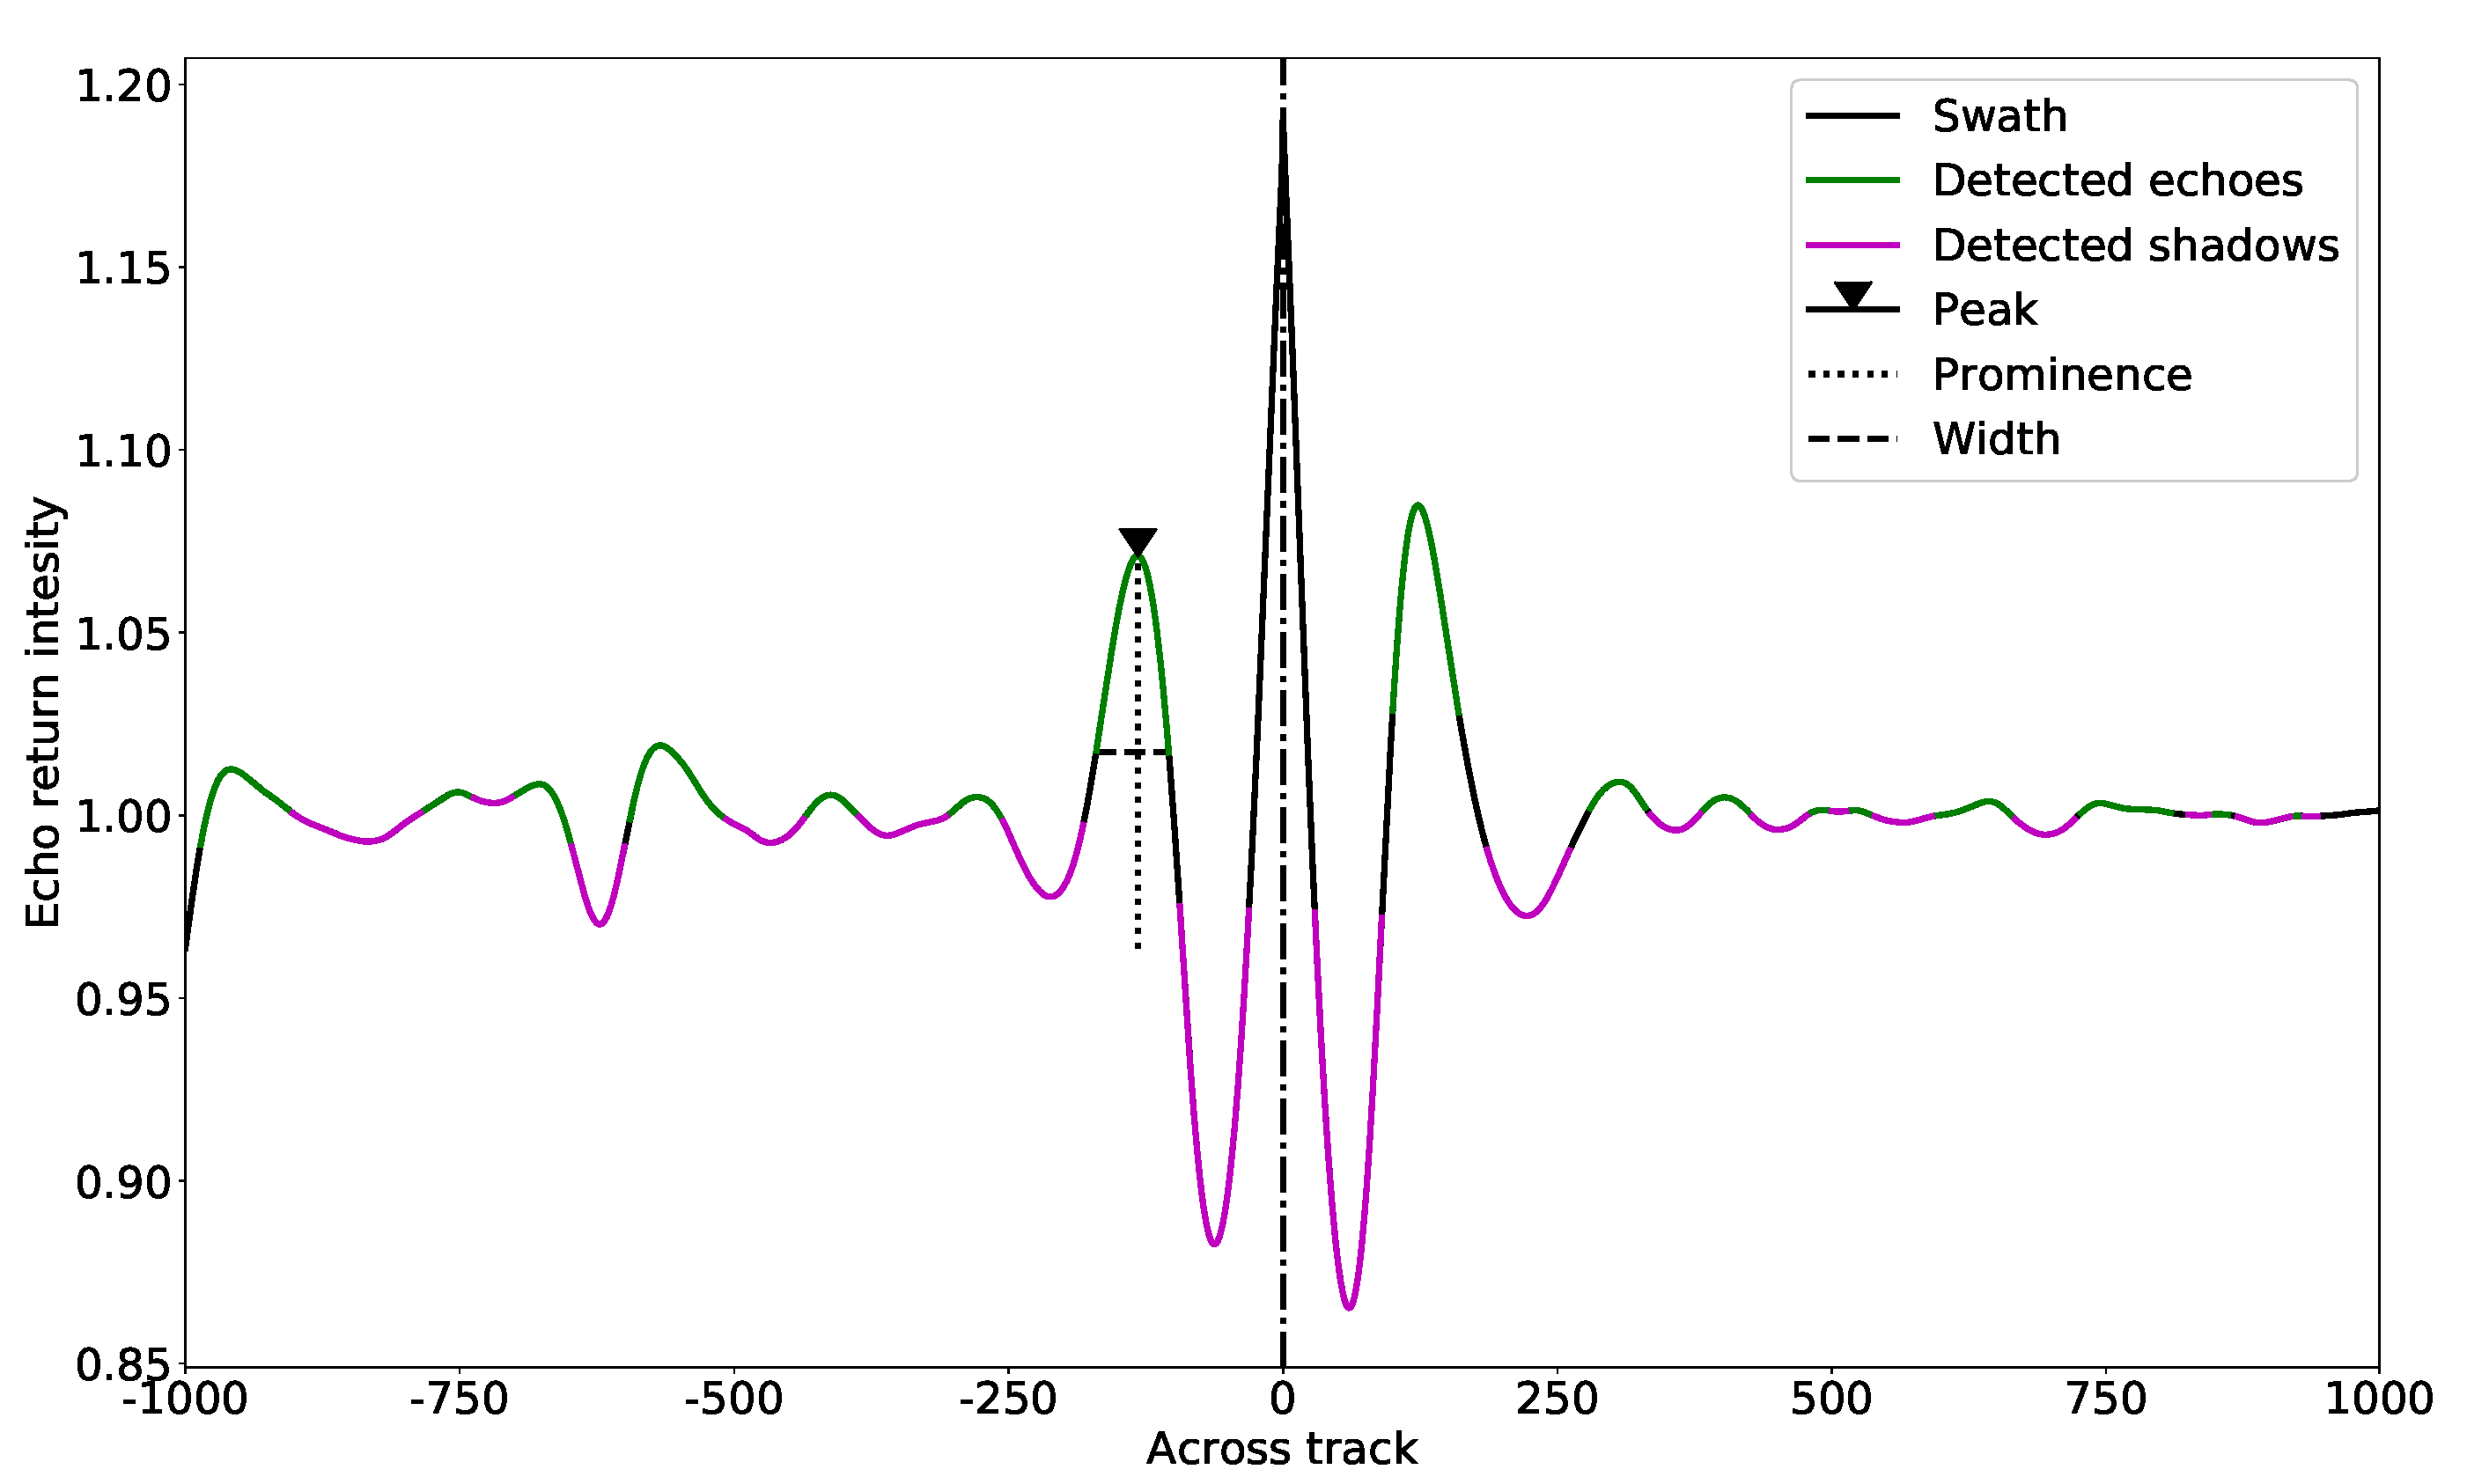
\includegraphics[width=0.8\textwidth]{figures/1D_swath_w_landmarks.eps}
    \caption{Normalized swath with all detected echoes and landmarks before filtering. The peak at the first bottom return for the left swath with its prominence and half-prominence width is also shown.}
    \label{fig:1D_swath_w_landmarks}
\end{figure}

In \cite{Al-Rawi2017LandmarkImages}, un-normalized SSS data is used, but the use of normalized data is suggested as an improvement. This report will present the result of performing landmark detection on normalized and unnormalized data. In addition, further improvements are suggested by applying morphological operators to remove thin landmarks and improve consistency. In the works of this report, a combination of a closing operation followed by an opening operation is tested on 2D binary images, constructed of shadows and echoes from the result of detecting landmarks in normalized data. 

\section{2D landmark detector using expert rules}

The 2D landmark detector, as in \cite{Leblond2019SonarProject}, finds shadows by intensity thresholding and uses a set of rules to filter out the shadows of the right size and shape. The first step is to perform an intensity thresholding on all the pixels to find shadows. The suggested intensity threshold is

\begin{equation}
    t_i = \frac{\Bar{I(x,y)}}{2},
    \label{eq:orginal_int_thres}
\end{equation}

where $\Bar{I(x,y)}$ is the average pixel intensity in the sonar image. However, this threshold produced close to no shadows from the data, so a new intensity threshold is suggested

\begin{equation}
    t_i = [\Bar{I(x,y)} - I(x,y)_{min}] k_i + I(x,y)_{min},
\end{equation}

where $I(x,y)_{min}$ is the average over the $100$ pixels with the lowest intensity, which increases robustness. Here, $k_i$ is a tuning parameter ranging from $0$ to $1$. Using the result from the intensity thresholding, a series of filtering rules are applied to filter out shadows. First, the shadows get filtered based on how many swaths they span over, where both minimum and maximum height filtering is applied. Second, filtering based on the area of the shadows in $pixels^2$ is applied. To account for how the grazing angle affects the shadows, the area is corrected by

\begin{equation}
    A_{corr} = A_s \frac{r_{ob,min}}{r_{ob}},
    \label{eq:corrected_area}
\end{equation}

where $r_{ob, min}$ is a reference object ground range that is tuneable, $r_{ob}$ is the ground range to the object, and $A_s$ is the area of the shadow in $pixels^2$. The last step is to filter the shadows based on how much of the bounding box that surrounds them that are filled, where the fraction of the filled area is given by

\begin{equation}
    \frac{A_s}{A_{bb}},
    \label{eq:fill_rate_bb}
\end{equation}

where $A_{bb}$ is the area of the bounding box surrounding the shadow. The bounding box's fill rate is compared to the fill rate threshold, $t_{fr}$. In addition to the proposed rules and tuning parameters, this report adds a closing operation to generate consistent landmarks. The structuring element (SE) is restricted to be quadratic, giving a new tuning parameter, $s_c$, for the size of the quadratic structuring element used for the closing operation. \cref{tab:2D_tuning_rules} summarises all tunable parameters and corresponding filtering rules. 

\begin{table}
    \begin{center}
    \caption{The table shows all the tunable parameters for the 2D landmark detector and the corresponding filtering rules applied.}
    \begin{tabular}{ll}
        \hline
        \textbf{Tunable parameter} & \textbf{Filtering rule}                            \\ \hline
        $k_i$             & $I(x,y) < (\Bar{I(x,y)} - I(x,y)_{min}) k_i + I(x,y)_{min}$ \\ 
        $s_c$             & Morphological closing on the shadows with SE of size $k_c$  \\ 
        $n_{swaths,min}$  & $n_{swaths} > n_{swaths,min}$                               \\ 
        $n_{swaths,max}$  & $n_{swaths} < n_{swaths,max}$                               \\ 
        $r_{ob,min}$      & $A_{corr} = A_s\frac{r_{ob,min}}{r_{ob}}$                   \\ 
        $A_{min}$         & $A_{corr} > A_{min}$                                        \\ 
        $t_{fr}$          & $\frac{A_s}{A_{bb}} > t_{fr}$                               \\ 
        \hline
    \end{tabular}
    \end{center}
    \label{tab:2D_tuning_rules}
\end{table}

\section{Qualitative comparison}

This report makes a qualitative comparison of the landmark detectors' results to compare them against each other. To make a meaningful comparison, some grounds for comparison must be set. First and foremost, an understanding of what part of a sonar image is considered a landmark and what is just considered background is needed. Next, an understanding of what makes up consistent landmarks is also essential. Lastly, some grounds for comparing the tuning process have to be defined. 

To compare the methods, understanding what parts of the sonar image are actual landmarks and what properties are consistent with a landmark is needed. Firstly, a division into echo and shadow landmarks has to be done. Echoes are typically generated by objects standing out from the seafloor, reflecting more sound and generating a more significant echo intensity in the sonar image. On the other hand, shadows are generated by occlusion, either by objects on the seafloor or simply by holes at the seafloor, and give dark areas in the sonar image. In the context of SLAM, landmarks that are re-detectable with different gracing angles and heading angles are of interest, and this should be the primary objective. However, it is not trivial to point out the properties such landmarks will have. 

\cref{fig:object_shadow} shows the same object being observed with two different gracing angles, $\theta_{s,1}$ and $\theta_{s,2}$. The shadow sizes and the grey unknown areas are inverse-proportional to the gracing angle. As the grey areas are unobserved, the backside of the landmark is unknown, and there could even be a second, smaller landmark behind the detected landmark. Since the backside is unknown, it is hard to make assumptions about the echo of the landmark observed with a different heading angle. However, inferring this to how the shadow appears is easier since the front is known. In that sense, shadow landmarks are preferred over echo landmarks. Further, small landmarks are unwanted because they can easily be occluded or mistaken by noise. Large landmarks are also unwanted. This is because they might be only partially observed in one situation and then fully observed in the next, making data association hard. 

\begin{figure}
    \centering
    \includegraphics[width=0.7\textwidth]{figures/object_shadow.drawio.pdf}
    \caption{The figure shows how the same object, observed with two different gracing angles, generates different-sized shadows and that both the grey unknown areas and the shadow sizes are inverse-proportional to the gracing angle.}
    \label{fig:object_shadow}
\end{figure}

Landmark consistency is an essential qualitative measure and tells to what extent a landmark detection method can detect a landmark as one coherent landmark or several minor landmarks. The opposite is when what appears as one consistent landmark in the sonar image is either only detected partially or as several minor landmarks. The problem with partially detected or split landmarks is that small changes in how the landmark is observed can result in a landmark with a widely different form or size being detected. This, again, can lead to problems for the data association. 

Another vital measure when comparing landmark detection methods is how sensitive, complex, and intuitive the detector tuning is. Sensitivity is vital because if a method has a significant sensitivity, small changes in the operating conditions can significantly change performance. On the other hand, if the method has an acceptable performance over a wide range of parameters, it is more likely that the same is evident over a wide range of operating conditions. Next, the complexity of the tuning says something about how difficult it is to obtain good results and how interconnected the different parameters are in each other. Suppose the parameters do not have a great deal of interconnection. In that case, it is possible to tune one parameter at a time sequentially and end up with acceptable performance. In the opposite case, tuning one parameter will significantly influence the other parameters' effect on the performance, making it more difficult to obtain acceptable performance. Hence, the tuning is more complex. Last, how intuitive a tuning process is, is tightly related to the interpretation of the tuning parameters. If the parameters are only arbitrary sizes, their effect on the performance is generally less likely to be intuitive. On the other hand, the tuning can be said to be more intuitive if there is a direct relation between the parameters and the effect they have on the performance.     

\chapter{Results}

This chapter will present results from testing the two landmark detector methods and the quality indicator on SSS data. The data was acquired in the Trondheims fjord by \textit{AURLab} using their vehicle \textit{LAUV Fridtjof} \cite{LAUVNTNU}. \cref{fig:neptus_screenshot} shows a map of parts of the Trondheim fjord and marks where the data was acquired, where the origo for the data is at N\ang{63;24;16.685} E\ang{10;24;5.8962}. Further, the data was divided into a training and a test dataset of $4890$ and $3000$ swaths, respectively. The training dataset was used to tune the landmark detectors, and the test dataset was used to evaluate their performance. 

\cref{fig:path_sonar_colorbars} shows the normalized training data. On the right is the path of the AUV shown, and in addition, is the distance traveled in the xy-plane shown along the path. Since the AUV is assumed to have an approximately constant altitude during the survey, altitude data is omitted. The same distance traveled is shown on the right in the sonar image. As the speed of the AUV changes throughout the data, so will the scaling of the distance traveled; hence, the ticks shown can be used to give some sense of the distances in the path and the sonar image but can not be used to accurately infer the distance traveled in between the ticks. 

\begin{figure} [h!]% order of priority: h here, t top, b bottom, p page
  \centering
  \includegraphics[width=0.84\textwidth]{figures/hercules_data.png}
  \caption{Map showing part of the Trondheim fjord and where the data used in this report was acquired. The zoomed-in path shows the path the AUV took during the data collection. }
  \label{fig:neptus_screenshot}
\end{figure}

The right side of \cref{fig:path_sonar_colorbars} shows the sonar image, the quality indicator, the speed of the AUV, and the color bar of the two latter. The right side of the sonar image indicates the distance traveled, and the left side the swath numbers, starting from swath number $0$. The swath numbers, unlike the distance traveled, scale linearly but do not have any relation to the sizes on the seafloor. On the x-axis are the bin numbers displayed, where the left part of the swath span from $0$ to $-1000$ and the right part from $0$ to $1000$. Since the mapping from bin numbers to seafloor metrics vary with altitude along the path, it is non-trivial to present it in an image like this; therefore, only the bin numbers are displayed. Investigating the sonar image closely, frequently occurring artificial lines going across the image can be observed. The same lines are more obvious in \cref{fig:1D_raw_tuning_training} due to the image not being normalized. The source of these lines is the transmission of acoustic messages between the AUV and a surface vessel. Further, the quality indicator is shown directly to the right of the sonar image in green-yellow-red colors, and its color scaling is shown on the far right of the figure. The interpretation of the quality indicator will be discussed below. On the right of the sonar image is the speed of the AUV in the xy-plane shown, and its color scaling is shown on the far right side. The color scaling of the quality indicator is the same throughout this report, but due to different speed ranges, the speed scaling differs between the training and test data. The color scaling for the test data is shown in \cref{fig:test_data}. 

\begin{figure}
    \centering
    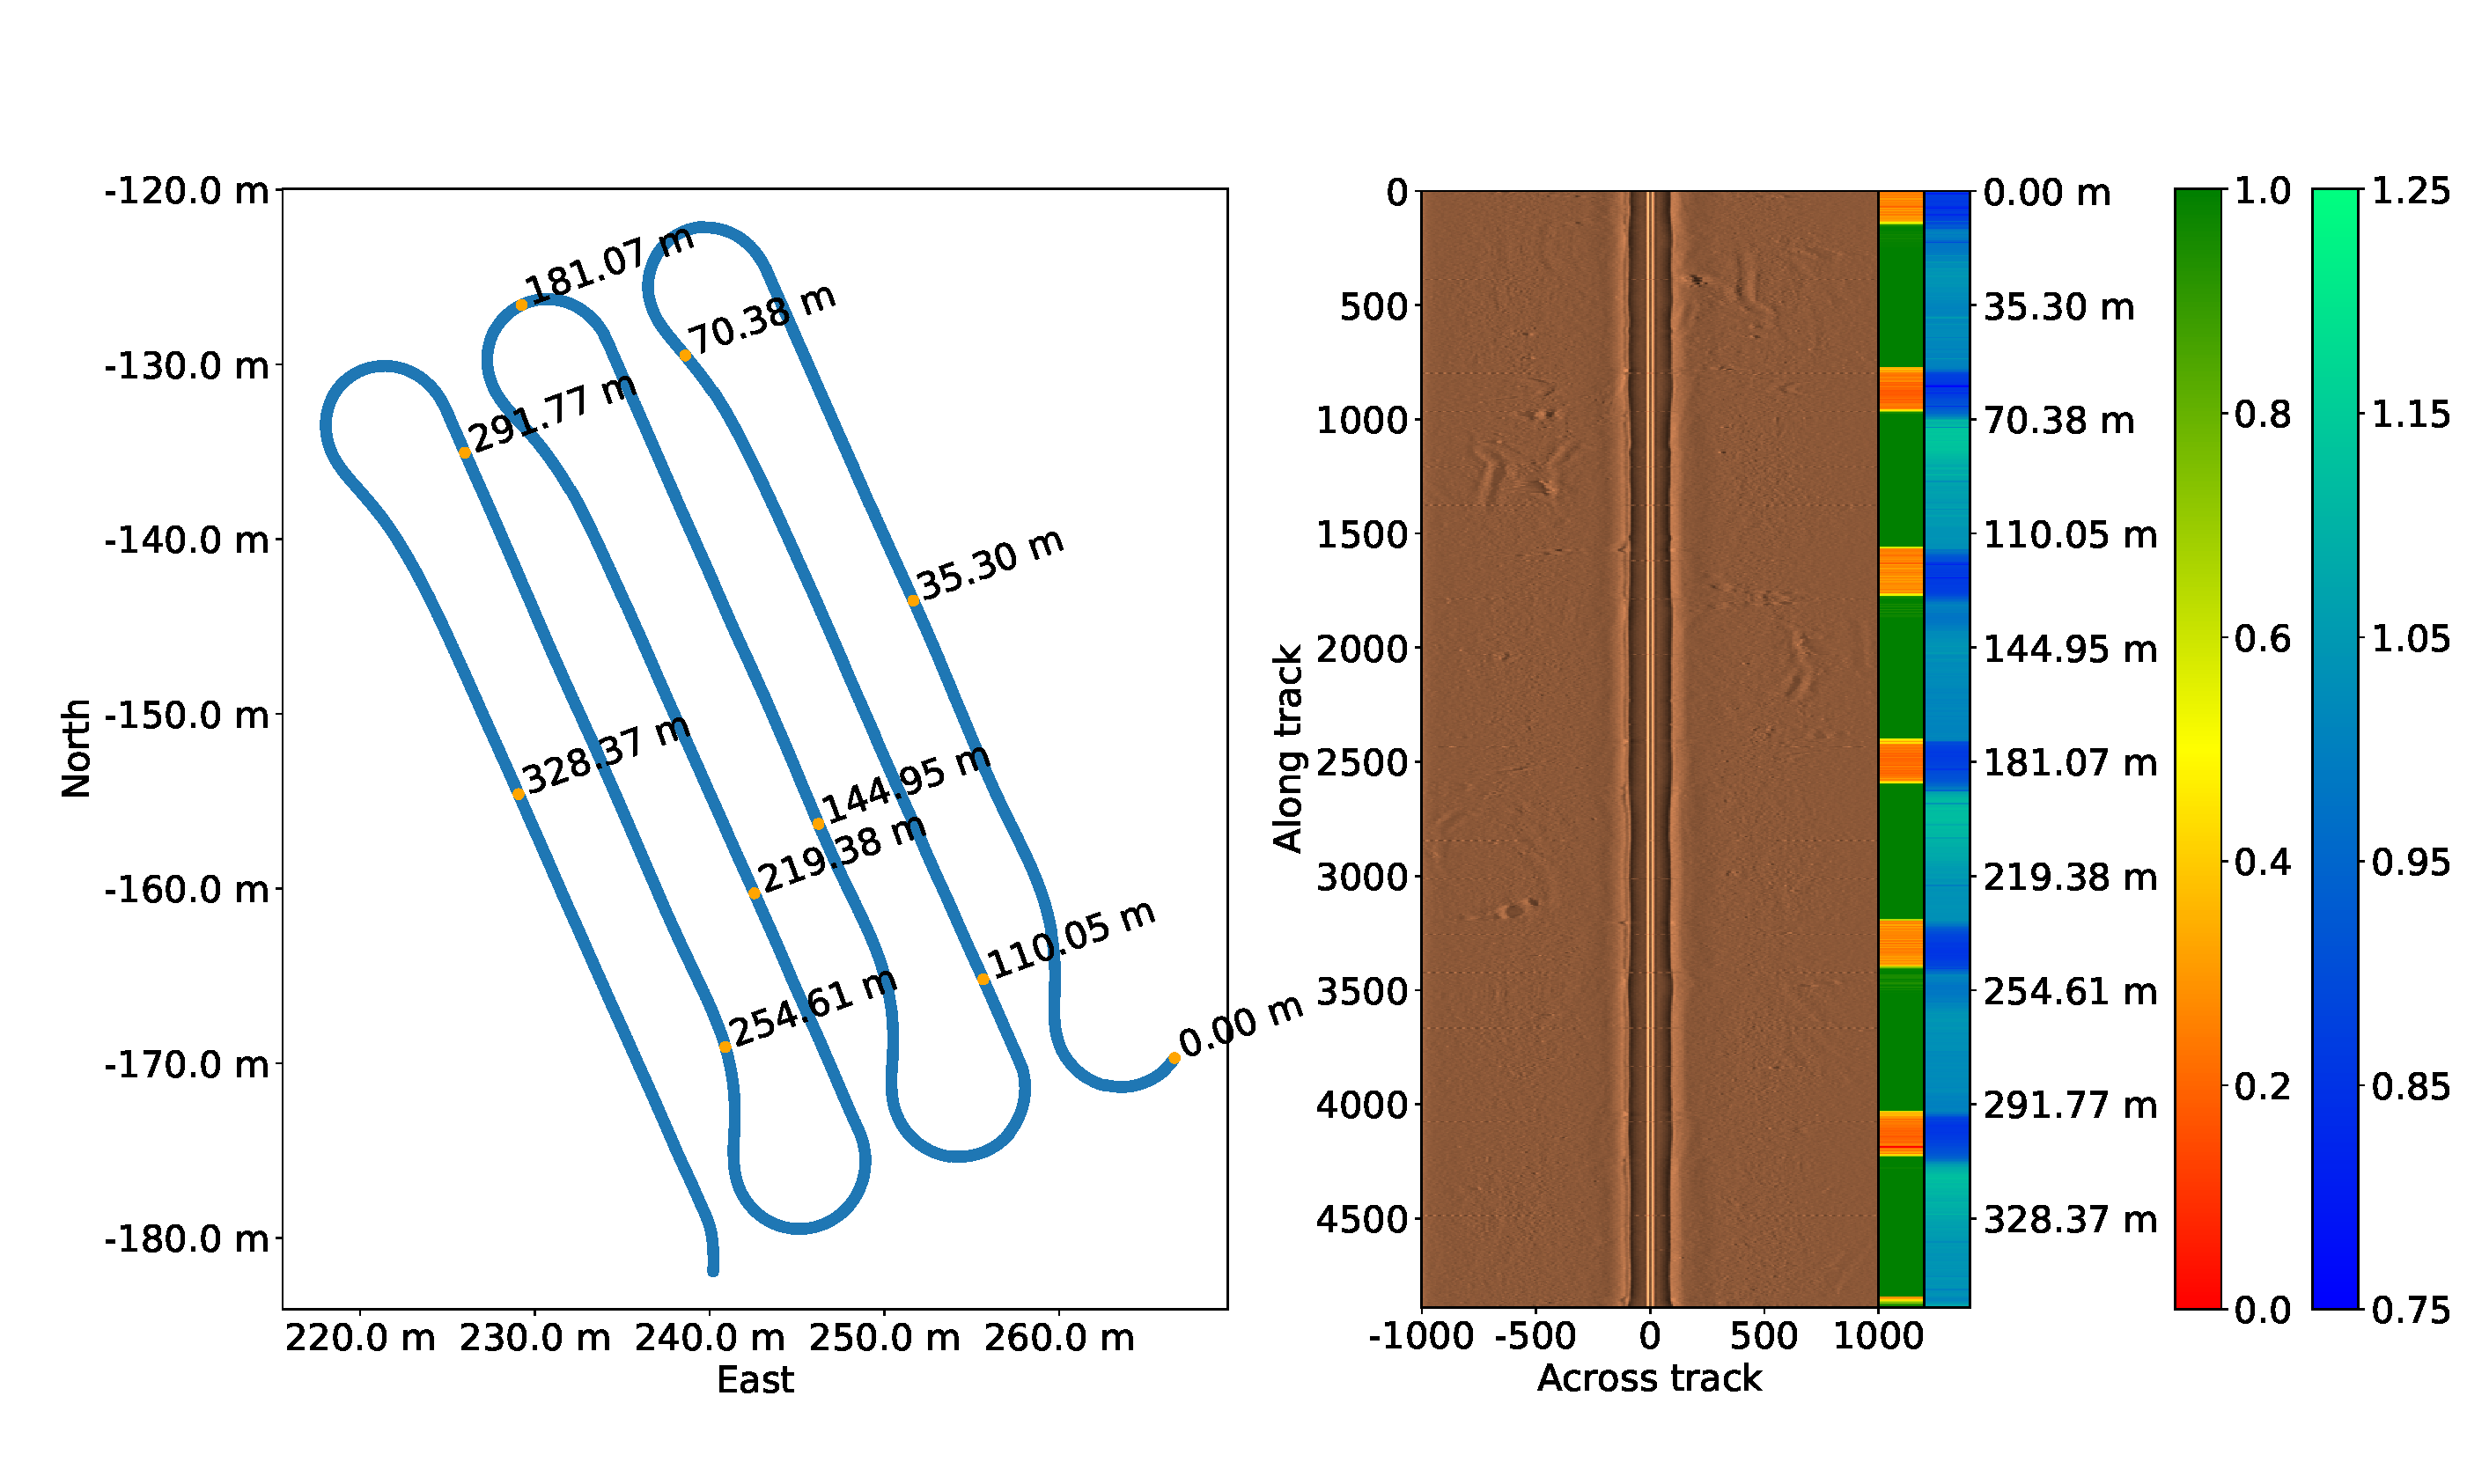
\includegraphics[trim=0cm 1.4cm 0cm 3.1cm, clip=true, width=1.0\textwidth]{figures/path_sonar_colorbars_training.eps}
    \caption{\textbf{Left:} The traveled path of the AUV from the training data set. In addition, the traveled distance is shown along the path. \textbf{Right:} The acquired normalized sonar image from the training data, with its corresponding quality indicator and speed in the xy-plane showed in direct relation, respectively. The color scaling of the quality indicator and speed used for all training data is shown on the far right.}
    \label{fig:path_sonar_colorbars}
\end{figure}

When tuning the landmark detector methods, the main objective was to have as few as possible false positives, the secondary to generate consistent landmarks, while the number of false negatives was only slightly considered during tuning. 

\section{Quality indicator for side scan sonar data}

The quality indicator is a measure that estimates the quality of the SSS data, an estimate that should be lower when turning due to overlapping swaths. \cref{fig:path_and_quality_ind} shows the result of testing the quality indicator on the training data, where the top left side is a plot of the path of the AUV in the xy-plane. Further, the quality indicator is overlayed as the color of the path. As expected, the data quality decreases when turning due to swath overlapping. In addition, the traveled distance in the xy-plane is also shown along the path. The acquired sonar data from traveling along the path is plotted on the right side, and the image's bars on the top right are the quality indicator and the speed of the AUV. The dashed horizontal lines in the image are displayed to show approximately in which part of the image the poor quality occurs. At a traveled distance of around $60 m$, two banana-like shadows appear. These could typically be examples of the anomalies and degradation of quality experienced when turning during a sonar survey. The bottom part of the figure shows a zoomed-in part of the path. The black lines correspond to the effective ground range, the ground range for the maximum sensor opening, for two and two consecutive swaths. For $q = 1.0$, the swaths do not overlap, but for $q = 0.54$ and $q=0.24$, the swaths overlap at the blue "x"s. 

\begin{figure} [h]% order of priority: h here, t top, b bottom, p page
  \centering
  \includegraphics[trim=0cm 0cm 0cm 0cm, clip=true, width=0.9\textwidth]{figures/quality_indicator_and_path.pdf}
  \caption[Path with quality indicator overlayed]{\textbf{Top left:} The traveled path in the xy-plane of the AUV. The path's color corresponds to the quality indicator along the path, and the traveled distance is also shown. \textbf{Top right:} The right figure shows the sonar image acquired from moving along the path and the corresponding quality indicator and speed of the AUV. \textbf{Bottom:} A zoomed part of the path where the quality indicator is displayed as the color of the path, and the black lines correspond to the effective ground range for two and two consecutive swaths. The blue "x"s marks were two consecutive swath overlaps.}
  \label{fig:path_and_quality_ind}
\end{figure}

\section{1D landmark detector using peak detection}

The 1D landmark detector has two tuning parameters, the threshold filtering the shadows and echoes, $E$, and the smoothing parameter, $p$, for the cubic spline smoothing the data. \cref{fig:1D_raw_tuning_training} shows the results from tuning, with three different thresholds represented, where the middle threshold of $E = 17$ was chosen. Even though there is not much difference between the different thresholds, there are some minor ones. For the threshold of $E = 16$, the clear shadow landmark around swath number $1300$ in the left swath loses some consistency compared to the chosen threshold of $E = 17$. For $E = 18$, two extra echo landmarks in the right swath around swath number $500$ were detected. The two extra detected landmarks are part of a larger landmark and are, together with the two connected shadow landmarks, an inconsistent detection of the landmark. A smoothing parameter of $p = \num{1e-5}$ was chosen to filter out noise to reduce the detection of false positives. Further, some false positives are detected, but all of these are in connection to the acoustic communication with a surface vessel and are therefore not considered. 

\begin{figure}   % order of priority: h here, t top, b bottom, p page
  \centering
  \includegraphics[width=1.0\textwidth]{figures/1D_raw_tuning_training.eps}
  \caption[Results of tuning threshold of the 1D method]{Results from tuning the thresholds of the 1D method with three different thresholds on unnormalized data. The left image shows the unnormalized training data without any landmark detection. The three other images show the results using a threshold $E = 16$, $E = 17$, and $E = 18$. All images are smoothed with a smoothing parameter of $p = \num{1e-5}$. Shadow landmarks are shown in green and echo landmarks are in pink. The two bars on the right show the quality indicator and the vehicle's speed.}
  % Parameters used: smoothing e-5
  \label{fig:1D_raw_tuning_training}
\end{figure}

\begin{figure} [ht!]
    \centering
    \includegraphics[trim=0cm 0cm 2.5cm 0cm, clip=true, width=0.8\textwidth]{figures/1D_result_training.pdf}
    \caption{\textbf{Left:} Result from tuning the 1D landmark detector on unnormalized training data with threshold $E = 17$. \textbf{Middle:} Result from tuning the 1D landmark detector on normalized training data with threshold $E = 1450$. \textbf{Right:} Results from tuning the 1D landmark detector on normalized training data with threshold $E = 1450$ and sizes for the quadratic structuring element of the closing and opening operation of $s_c = 10^2$ and $s_o = 15^2$, respectively. All results use a smoothing parameter of $p = \num{1e-5}$. The shadow landmarks are pink, and the echo landmarks are green.}
    \label{fig:1D_tuning_results}
\end{figure}

As suggested in \cite{Al-Rawi2017LandmarkImages}, using normalized data and morphological operators to filter out thin landmarks were tested, and \cref{fig:1D_tuning_results} shows the results. The left image results from using unnormalized training data with a threshold of $E = 17$, the middle image from testing the method on normalized data with $E = 1450$, and the right image are the results of applying a closing operation followed by an opening operation with quadratic structuring elements of sizes $s_c = 10^2$ and $s_o = 15^2$ on the middle image. Using the same considerations as when tuning the 1D landmark detector on unnormalized data, the threshold of $E = 1450$ was found. Again, all false positives are considered to originate from acoustic communication. The false positives are all echo landmarks and appear in pairs, one on the left side and one on the right side of the swath, and can be found approximately in swath numbers $1300$, $2000$, and $4200$. In addition, a few landmarks are inconsistently detected. For the right image, the sizes of the structuring elements were found by testing different sizes and choosing the ones that generated results most aligned with the tuning objectives. All false positives are removed, and the resulting landmarks are mostly consistent. Both the rightmost shadow landmark and the shadow landmark at around swath number $1200$ are part of a larger landmark and are inconsistently detected. All results were obtained using a smoothing parameter of $p = \num{1e-5}$. \cref{tab:1D_parameters} summarizes the parameters used. 

\begin{table} [h]
    \caption{Resulting parameters from tuning the 1D landmark detector on unnormalized and normalized training data.}
    \centering
    \begin{tabular}{cccc}
        \hline
        \textbf{Tunable parameter} & \textbf{Unnormalized} & \textbf{Normalized} & \textbf{Normalized with morph. operators} \\ \hline
        $E$                        & $17$                  & $1450$              & $1450$                                    \\
        $p$                        & $\num{1e-5}$          & $\num{1e-5}$        & $\num{1e-5}$                              \\
        $s_c$                      & $-$                   & $-$                 & $10^2$                                    \\
        $s_o$                      & $-$                   & $-$                 & $15^2$                                    \\ \hline
    \end{tabular}
    \label{tab:1D_parameters}
\end{table}

\newpage
 
Comparing the results in \cref{fig:1D_tuning_results}, there is not much difference in performance in the left and middle images using unnormalized and normalized data. However, as discussed in \cref{sec:disc_1D_landmark_detector}, normalized data is preferred over unnormalized data. Further, using morphological operators on normalized data gives significantly better results than without and is therefore chosen to compare against the 2D landmark detector.

\section{2D landmark detector using expert rules}

The 2D landmark detector has a total of six parameters to tune. The parameter $r_{ob, min}$ was set to $3 m $, as in \cite{Leblond2019SonarProject}. \cref{fig:2D_tuning_intensity_thres} shows the result from tuning the intensity threshold with three different intensity thresholds displayed, where the intensity threshold of $k_i = 0.9$ was chosen. An intensity threshold of $k_i = 0.85$ results in less noise in the detected landmark candidates than the chosen threshold of $k_i = 0.9$. However, landmark candidates without a strong shadow are not detected consistently. Several large landmark candidates either have holes or are not consistently detected. An intensity threshold of $k_i = 0.95$ results in much more noise in the detected landmark candidates, which is unwanted. An intensity threshold of $k_i = 0.9$ produces consistent landmark candidates and an acceptable amount of noise. 

\cref{fig:2d_tuning_paramaters_training} shows the results of tuning the last four parameters. The green landmark candidates are the landmarks filtered out in the corresponding step of the pipeline, and the pink landmarks are the kept landmarks. The leftmost image shows the sonar image. The second leftmost image results from filtering landmark candidates by how many swaths they are a part of, i.e., the height of the landmark candidate in the sonar image. The landmark candidates are generated by applying intensity thresholding on the sonar image. Large landmarks are chosen to be filtered out because it is more difficult to detect them consistently, and therefore a more conservative choice is made. The minor landmarks were also filtered out, resulting in $n_{swaths, min} = 50 \; swaths$ and $n_{swaths, max} = 150 \; swaths$. In addition, this step filters out much of the noise in the landmark candidates. The third image shows the result of applying the landmark area filtering. The parameter $A_{min} = 100 \;pixels^2$ was chosen to filter out the minor landmarks left from the height filtering. The fourth image shows the result of filtering out landmarks based on their fill rate of the rectangular bounding box encapsulating them. The fill rate limit was set to $t_{fr} = 0.3$ to filter out the thin and non-consistent landmarks. The last image shows the resulting landmarks.

Looking at the height filtering step in \cref{fig:2d_tuning_paramaters_training}, it is evident that two of the inconsistently detected landmarks (landmark number two and three from the top) are so because they are split by artifacts occurring from acoustic communication. Drawing from the 1D landmark detector, a closing operation with a quadratic SE of size $s_c = 10^2$ is added between the intensity threshold step and the height filtering. \cref{fig:2d_tuning_paramaters_w_filtering_training} shows the tuning of the pipeline. Due to the more consistent landmark candidates, the amount of noise could be reduced by reducing the intensity threshold to $k_i = 0.85$. The other parameters were not changed. The two landmarks inconsistently detected earlier are not detected and rightly removed due to their height. Further, two new landmarks are detected. The resulting parameters are shown in \cref{tab:2D_parameters}. Comparing with and without morphological operators, it is evident that the closing operation helps with consistency; therefore, this is the preferred method for comparing with the 1D landmark detector. 

\begin{figure}  % order of priority: h here, t top, b bottom, p page
  \centering
  \includegraphics[trim=0cm 1.6cm 0cm 1.4cm, clip=true, width=0.95\textwidth]{figures/2D_tuning_threshold_training.eps}
  \caption[Results of tuning intensity threshold the 2D method]{Results from tuning the intensity thresholds of the 2D method with three different thresholds on normalized data. The left image shows the normalized training data without any thresholding. The three other images show the results using an intensity threshold of $k_i = 0.85$, $k_i = 0.9$, and $k_i = 0.95$. All images are smoothed with a smoothing parameter of $p = \num{1e-2}$. Landmark candidates are shown in green. The two bars on the right show the quality indicator and the vehicle's speed.}
  \label{fig:2D_tuning_intensity_thres}
\end{figure}

\begin{table} 
    \caption{Resulting parameters from tuning the 2D landmark detector on normalized training data.}
    \centering
    \begin{tabular}{ccc}
        \hline
        \textbf{Tunable parameter} & \textbf{Normalized} & \textbf{Normalized with morph. operators} \\ \hline
        $k_i$                      & $0.9$               & $0.85$                                    \\
        $s_c$                      & $-$                 & $10^2$                                    \\
        $n_{swaths, min}$          & $50 \; swaths$      & $50 \; swaths$                            \\
        $n_{swaths, max}$          & $150\; swaths$      & $150 \; swaths$                           \\
        $r_{ob, min}$              & $3 \; m$            & $3 \; m$                                  \\ 
        $A_{min}$                  & $100 \; pixels^2$   & $100 \; pixels^2$                         \\
        $t_{fr}$                   & $0.3$               & $0.3$                                     \\ \hline
        
    \end{tabular}
    \label{tab:2D_parameters}
\end{table}

\begin{figure} % order of priority: h here, t top, b bottom, p page
     \centering
    \begin{subfigure}[t]{0.975\textwidth}
        \centering
        \includegraphics[trim=0cm 3cm 0cm 2.8cm, clip=true, width=\textwidth]{figures/2D_tuning_parameters_training.eps}
        \caption{Results from tuning the 2D method on normalized data. An intensity threshold of $k_i = 0.9$ generates the landmark candidates used.}
        \label{fig:2d_tuning_paramaters_training}
     \end{subfigure}
     \hfill
     \begin{subfigure}[b]{0.975\textwidth}
        \includegraphics[trim=0cm 3cm 0cm 2.8cm, clip=true, width=1.0\textwidth]{figures/2D_filtered_tuning_parameters_training.eps}
        \caption{Results from tuning the 2D method on normalized data, using a closing operation to filter the landmark candidates. An intensity threshold of $k_i = 0.85$ followed by a closing operation with a quadratic SE of size $s_c = 10^2$ generates the landmark candidates used.}
        \label{fig:2d_tuning_paramaters_w_filtering_training}
     \end{subfigure}
        \caption{Results from tuning the 2D method on normalized data. In both figures, the left image shows the normalized training data without any detection. The four other images show the different steps in the pipeline, applying the different thresholds to the landmark candidates. The green landmark candidates are the landmarks filtered out in the corresponding step of the pipeline, and the pink landmarks are the kept landmarks. The two bars on the right show the quality indicator and the vehicle's speed.}
\end{figure}

\newpage

\section{Landmark detection on test data}

Both landmark detector methods were run on the test dataset to evaluate the performance of the landmark detectors with the chosen tuning parameters. \cref{fig:test_data} shows the test data. The result from the 1D landmark detector is shown in \cref{fig:1D_norm_result_test}. No false positives are detected; however, several landmarks are only partially detected. It is also worth noting that only one echo landmark is detected. \cref{fig:2D_result_single_test} shows the result from the 2D landmark detector. The conservative tuning is evident in the result, as several large, thin landmarks at the top of the image are not detected. Further, the two thin landmarks that are detected are only partially detected. 

\begin{figure} [hb] % order of priority: h here, t top, b bottom, p page
     \centering
    \begin{subfigure}[t]{0.87\textwidth}
         \centering
         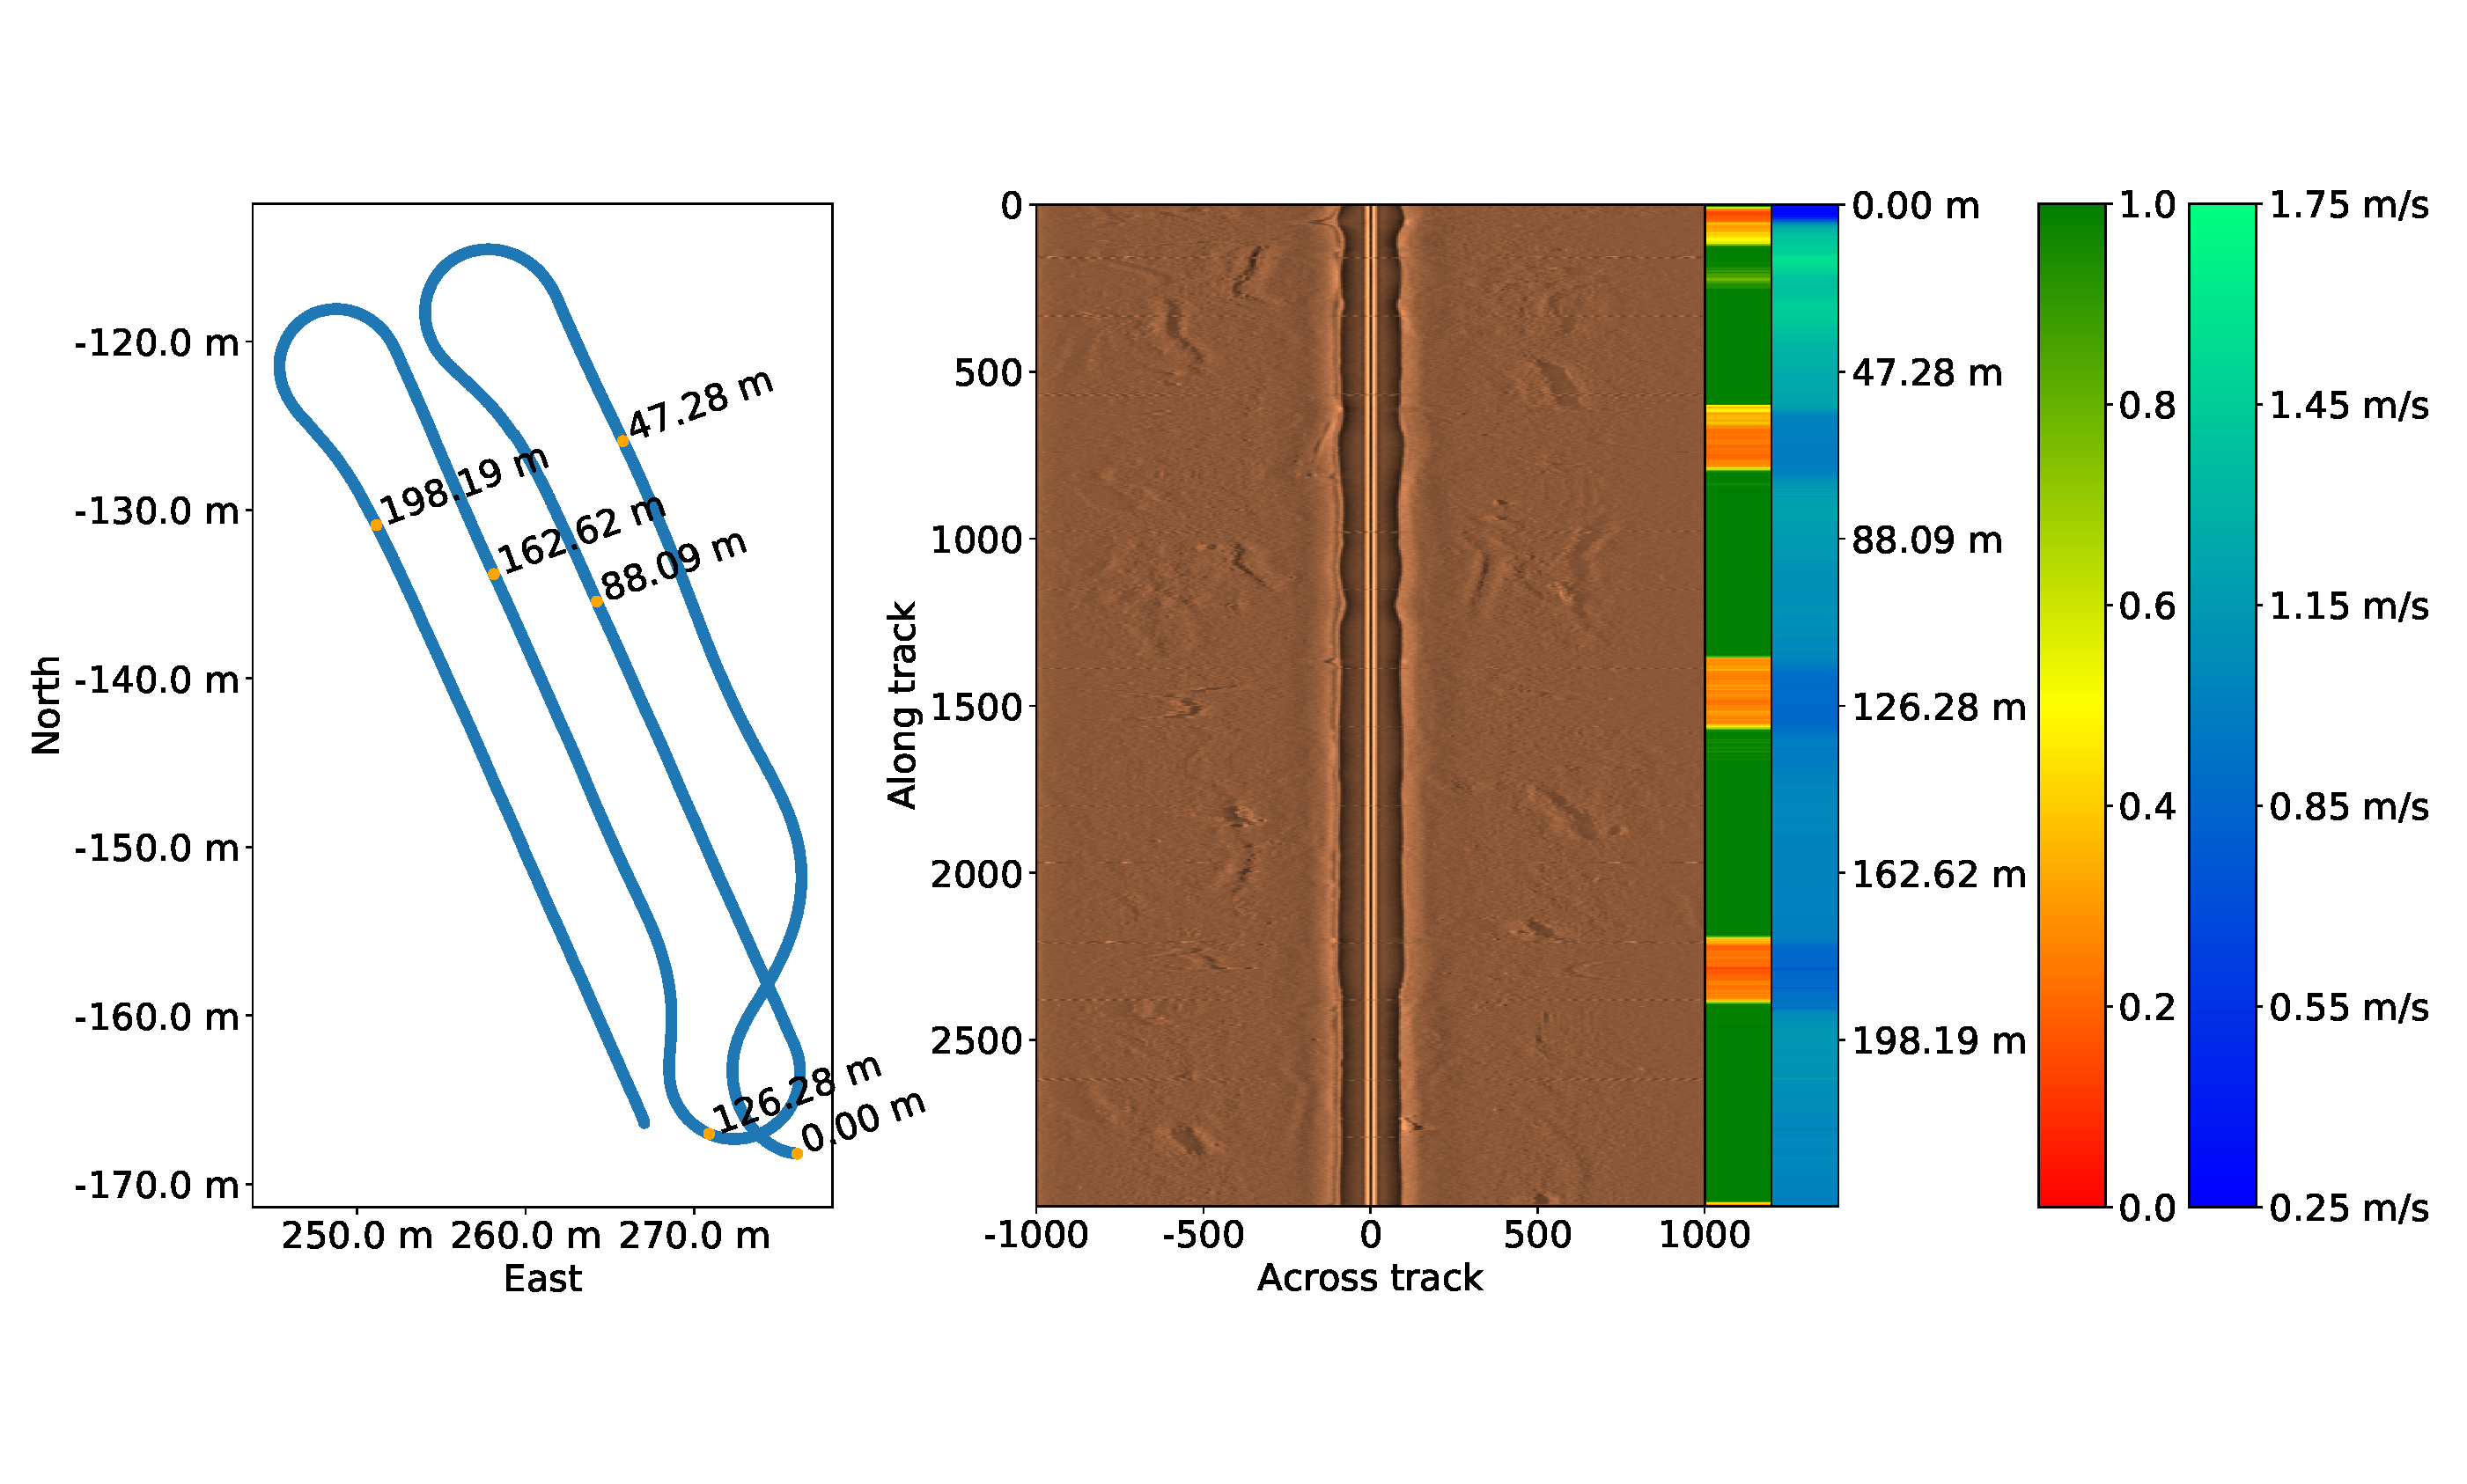
\includegraphics[trim=0cm 3.4cm 0cm 3.4cm, clip=true, width=\textwidth]{figures/path_sonar_colorbars_test.eps}
         \caption{\textbf{Left:} The traveled path of the AUV from the test data set. In addition, the traveled distance is shown along the path. \textbf{Right:} The acquired normalized sonar image from the test data with its corresponding quality indicator and speed of the AUV in the xy-plane showed in direct relation, respectively. The color scaling of the quality indicator and speed used for all test data is shown on the far right.}
         \label{fig:test_data}
     \end{subfigure}
     \hfill
     \begin{subfigure}[b]{0.44\textwidth}
         \centering
         \includegraphics[trim=9cm 1cm 10cm 1cm, clip=true, width=\textwidth]{figures/1D_norm_result_test.eps}
         \caption{1D landmark detector. Green is echo landmarks, and pink is shadow landmarks.}
         \label{fig:1D_norm_result_test}
     \end{subfigure}
     \begin{subfigure}[b]{0.44\textwidth}
         \centering
         \includegraphics[trim=9cm 1cm 10cm 1cm, clip=true, width=\textwidth]{figures/2D_result_single_test.eps}
         \caption{2D landmark detector. Pink is the detected landmarks.}
         \label{fig:2D_result_single_test}
     \end{subfigure}
        \caption{The test data represented and the results from running landmark detectors on the test data.}
        \label{fig:landmark_detection_test_data}
\end{figure}

\chapter{Discussion}

This chapter will discuss the results from the proposed landmark detectors and the quality indicator. In addition, a comparison of the two landmark detectors will be presented. 

\section{Quality Indicator for Side Scan Sonar}

The proposed quality indicator can give a good indication of how turning the AUV affects the quality of the SSS data, and it is evident in the data that there are fewer landmarks at the turning places and that the few landmarks are distorted by the motion of the AUV. In the right part of \cref{fig:path_and_quality_ind}, the black lines loosely divide the sonar image into good and poor-quality parts. The first to notice in the parts of poor quality, most of the landmarks appear to be, as expected, distorted. At around a traveled distance of $60 m$, a banana-formed landmark appears in both the left and right swath. Again at a traveled distance of about $180 m$, a weak banana-formed landmark appears again in the right swath. In the left swath, a more extended landmark and two small landmarks appear. It is hard to tell whether or not the more extended landmark is distorted, but the two small landmarks do not appear distorted. Here the quality indicator is of good help, pointing out that these landmarks most likely will have some distortions. 

Even though the quality indicator can point out where distortion and poor quality can appear due to swath overlapping, it will to a lesser degree, be able to point out if we will experience distortions due to weak turning, change in speed, or a change in roll angle. Looking at \cref{fig:path_and_quality_ind} again, we can see that after turns one and three, there is a section where the AUV is straightening up and performing a weaker turn to approach its path. Looking at the corresponding parts of the right-side sonar image, it is evident that the image appears torn and much of the contrast disappears, especially in the left swath. The quality indicator marks a few swaths as weak yellow, but it is not a clear indicator of the torn image. In addition, since speed is not directly incorporated and roll isn't incorporated in the quality indicator, it will not be able to detect distortions from changes in these. 

\section{1D Landmark Detector using Peak Detection}

As shown in \cref{fig:1D_norm_result_test}, the 1D landmark detector can detect some landmarks consistently, but most are not consistently detected. The top six landmarks are not close to being consistently detected. For the last six at the bottom, two landmarks are not consistently detected, giving only a third of the detected landmarks are considered consistent. If this landmark detection method should be used for SLAM, the data association would likely struggle to provide suitable landmark matches. 

Further, to keep the false positive rate small, much of the geometrical details and information are filtered out, not providing much more information than the position of the landmarks and, to some extent, their size. Depending on the application, this can be sufficient. Still, the landmark detector should be able to extract as much information from the landmarks as possible, as this applies to all applications. 

The process of tuning the 1D landmark detector was complex due to the parameters being tightly coupled and unintuitive since there was no direct relation between the threshold parameter and the desired properties of the detector. The latter can be seen in \cref{fig:1D_norm_tuning_training}, where three different thresholds are shown, and compared to the chosen threshold of $1550$, a threshold of $1600$ makes some of the landmarks more consistent but also introduces a new landmark that is not consistently detected. On the other hand, with a threshold of $1500$, only one landmark is removed, but the others do not seem to get more consistent. Throughout the tuning process, it became evident that it was very hard to sort out the landmarks of the desired size, as both small and large landmarks were added or removed if the threshold was altered. It was also evident that there was a tight coupling between the smoothing parameter and the threshold. A change in the smoothing parameter implied that the range where the threshold parameter gave somewhat acceptable results vas drastically change, making the tuning more complex. 

To sum up, the 1D landmark method cannot detect landmarks consistently and, at the same time, produce an acceptable amount of false positives and is, therefore, not usable in any practical application. In addition, its tuning process is complex and unintuitive, and the best parameter set found filtered out a lot of the geometrical information about the landmarks. 

\section{2D Landmark Detector using Expert Rules}

As shown in \cref{fig:2d_result_test}, the 2D method can, to a larger extent, detect consistent or near-consistent landmarks in the data, but not all detected landmarks are consistent. From the top, the two first landmarks can be said to be somewhat inconsistently detected, but it can be argued that at least the landmark closest to the AUV is close to consistently detected. It appears that the landmark is part of a larger landmark, but by close inspection, it is not clear what is the actual landmark. In addition, landmark number four from the top appears to be close to consistent. However, it is hard to point out what would be the ground truth landmark. The remaining landmarks are consistently detected. Therefore, even though not all landmarks are detected perfectly consistently, the method overall shows acceptable performance.

The tuning process is simple and mostly intuitive, as shown in \cref{fig:2D_tuning_intensity_thres} and \cref{fig:2d_tuning_paramaters_training}, and we can easily tune the different parameters to filter out the landmarks with the wanted geometrical properties. Because of the sequential inner workings of the detector, the tuning can also be done sequentially, making it possible to tune one parameter at a time. First, the intensity is tuned to pick out all landmarks consistently, together with an acceptable amount of false positives. How different thresholds effect the consistency and amount of false positives are easily observed in \cref{fig:2D_tuning_intensity_thres}. Next, the different geometrical parameters can be tuned to filter out the landmarks with the desired geometrical properties. Both the height parameters and the fill rate threshold are easily interpretable, and it is easy to predict their effect on the results. The area filtering is a bit more complex, as the area is corrected for the effect of the grazing angle. It is, therefore, not perfectly intuitive how it will affect the landmarks because its effect varies with how far the landmarks are from the AUV. However, producing an acceptable result without intuition about how the parameter affected the result is not difficult. All in all, the tuning can be said to be simple and mostly intuitive. 

To conclude, the 2D landmark detector produces acceptable results and possesses properties that make it simple and intuitive to tune, but it has some weaknesses regarding consistent landmark detection. Further work could improve the latter by doing a new local detection around each detected landmark with a relaxed intensity threshold to improve consistency.

\section{Comparison}

Both landmark detection methods can do detection with an acceptable level of false positives but suffer, to a varying degree, from not being able to detect the detected landmarks consistently. The 1D landmark detector struggles much more with consistently detecting landmarks than the 2D landmark detector and is considered unable to use in a practical application. The 2D landmark detector, on the other hand, has a much better performance and the potential to be used in practical applications.  However, inconsistent landmarks detection will make it much more challenging to apply in a SLAM context.

Even though the 2D landmark detector has twice as many tuning parameters, it is less complex and more intuitive to tune than the 1D landmark detector. This comes from the sequential inner workings and the non-dependent tuning parameters. The tuning is also worth considering for practical applications and, again, has the 2D landmark detector potential for being used in a SLAM context. 

\chapter{Conclusion}

The quality indicator is only able to point out where the sonar image is of bad quality but does not solve the problem.



\chapter*{\bibname}
\printbibliography[heading=none]

\appendix


\end{document}
